\paragraph{Mise en place de l'environement}:\\

Avant de commencer l'implémentation de notre programme, il a d'abord fallut mettre en place l'environement cible pour notre exécution, en l'occurence ici la distribution ALMOS pour TSAR.\\

On commence donc par télécharger la dernière distribution stable d'ALMOS à l'adresse :\\
.\\
\begin{DDbox}{\linewidth}
\begin{lstlisting}[language=bash]
https://www-soc.lip6.fr/trac/almos/chrome/site/almos-tsar-mipsel-1.0.tbz2
\end{lstlisting}
\end{DDbox}
Ensuite, il faudra décompresser l'archive :\\
.\\
\begin{DDbox}{\linewidth}
\begin{lstlisting}[language=bash]
$ tar jxf almos-tsar-mipsel-1.0.tbz2
\end{lstlisting}
\end{DDbox}
Dans notre cas, on a eu quelques soucis liés à l'absence de packets dont dépendait l'utilisation du simulateur, on a donc eu à installer la liste de packets suivante :\\
.\\
\begin{DDbox}{\linewidth}
\begin{lstlisting}[language=bash]
libc6-i386 lib32stdc++6 lib32gcc1 lib32ncurses5 lib32z1 xterm
\end{lstlisting}
\end{DDbox}
Les répertoires importants dans notre cas sont :\\
\begin{DDbox}{\linewidth}
\begin{lstlisting}[language=C]
dans almos-tsar-mipsel-1.0
-> ./test/pf1 : // contient le makefile launcheur de TSAR ( make sim<nb_clusters> )
-> ./apps :     // repertoire contenant les sources de nos applications
\end{lstlisting}
\end{DDbox}

\paragraph{Description de l'application}:\\

DWC ( Distributed Words Counter ) est une application de comptage distribué de nombre de mots dans un texte. Le choix de cette application, est motivé par la nécessité d'avoir une application parallèle dont on évaluera la performance ( speedup ). Cette application sera écrite en C, et utilisera l'API POSIX Threads pour exprimer le traitement parallèle, elle suivra le schèma de traitement illustré par la figure :\\

\begin{center}
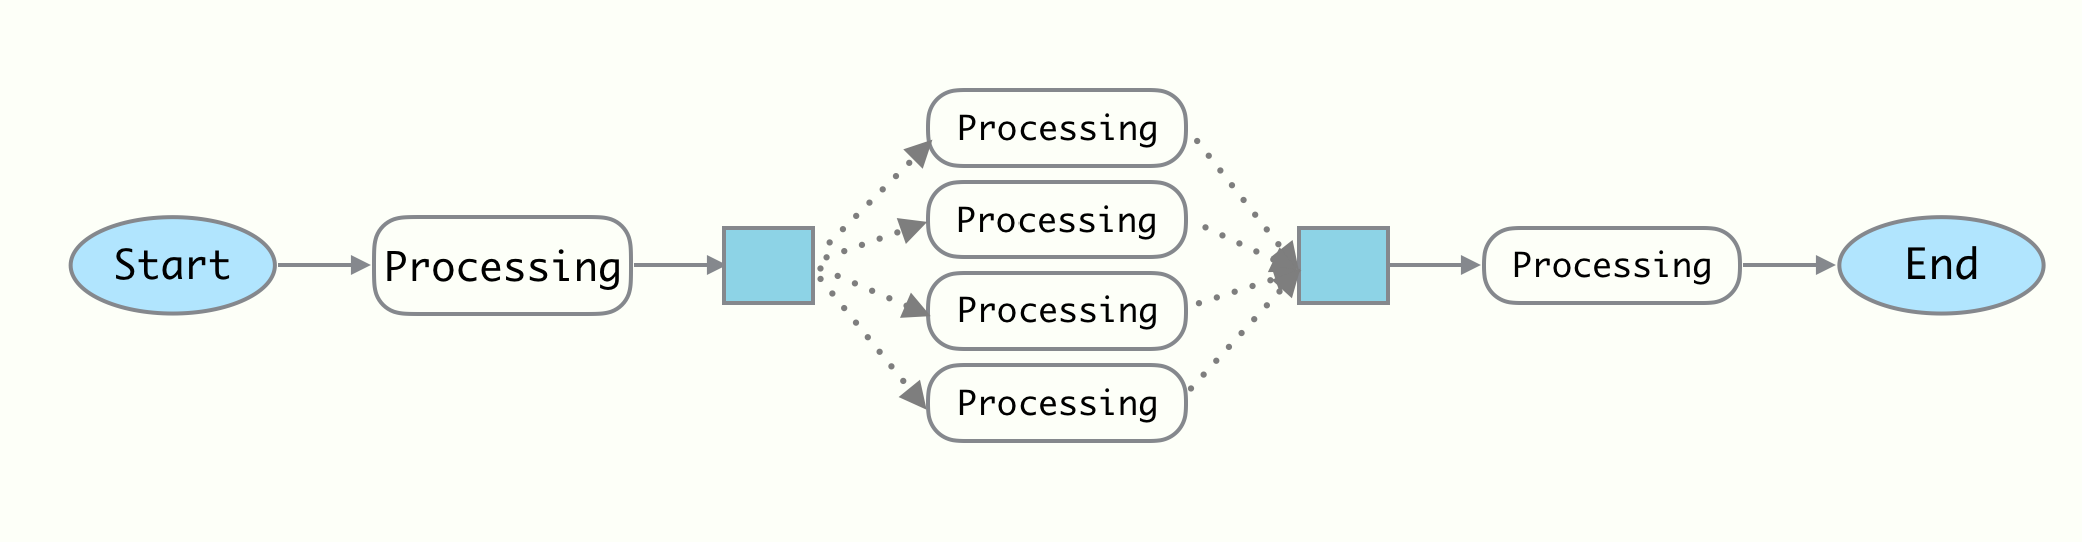
\includegraphics[scale=0.4]{images/processing.png}
\end{center}

La phase d'initialisation permet de remplir la structure de calcul, représentée dans notre cas par un tableau de mots générés aléatoirement et dont la taille sera définie à l'avance ( parce qu'on veut pouvoir manipuler la taille de mots, histoire de pouvoir évaluer les performances sur plusieurs plages de mots). On lancera ensuite autant de taches ``workers'' qu'il y a de processeurs dans la platforme matérielle, chaque tache ``worker'' aura sa plage de travail dans le tableau de mots, et produira un tableau correspondant au nombre de mots d'indice i du tableau de lettres. ( ainsi array[3] correspondra au nombre de mots de taille 3 ). Dès que les ``workers'' auront fini leur calcul, le main rentrera en phase de merge pour rassembler tous les tableaux de résultats et faire les sommes de nombres de mots.\\

Une exécution de l'application rend le temps de traitement en nombre de cycles par phase du programme. on exécutera le programme, sur les mêmes données et pour la même configuration séquentiellement et de manière distribuée ( pour les benchs ).\\

\paragraph{Notre rendu}:\\

L'archive rendue contient :\\
.\\
\begin{DDbox}{\linewidth}
\begin{lstlisting}[language=C]
-> ./apps/dwc/* // sources du programme dwc
-> ./apps/dwc/makefile // makefile le compilant
-> ./execMe.sh // script compile le programme et lance une serie de simulations comme decrit dans le paragraphe precedant
\end{lstlisting}
\end{DDbox}
Cette archive est à copier à la source de la distibution, c'est à dire dans le dossier almos-tsar-mipsel-1.0.
